\section{Numerik nichtlinearer Gleichungen und Gleichungssysteme}
\subsection{Grundlagen}
Ziel: Gesucht $x^* \in M \subset \rn$, so dass $f(x^*) = 0$ wobei $f: M \rightarrow \rn$\\
($ h(x) = g(x) \Leftrightarrow f(x) := h(x) - g(x) = 0$)\\
Typische ``numerische'' Vorgehensweise:
\begin{align*}
  f(x) = 0 \overset{G(x) \neq 0}{\Leftrightarrow} -G(x)f(x) = 0 \Leftrightarrow \underbrace{x - G(x)f(x)}_{=: \Phi(x) \text{ Fixpktglg}} = x
\end{align*}
Fixpunktiteration: $x^{(k+1)} = \Phi(x^{(k)})$\\
Fragestellungen:
\begin{itemize}
  \item Konvergenz
  \item Konvergenzbereich (für welche $x^{(0)}$ konvergiert die FPI?)
  \item Konvergenzgeschwindigkeit
\end{itemize}
\definition: Sei $M \subset \rn,\;\Phi: M \rightarrow \rn,\;\Phi(x^*) = x^* \in M$ und $x^{(k+1)} := \Phi(x^{(k)})$\\
Die Folge $(x^{(k)})_{k \in \mathbb{N}_0}$ heißt
\begin{itemize}
  \item global konvergent, falls $\mathbin{\textcolor{rot}{\forall\;x^{(0)} \in M}}: \underset{k \rightarrow \infty}{\lim} x^{(k)} = x^*$
  \item lokal konvergent, falls $\exists\;\epsilon > 0 \quad \mathbin{\textcolor{rot}{\forall\;x^{(0)} \in U_\epsilon(x^*)}}: \underset{k \rightarrow \infty}{\mathrm{lim}} x^{(k)} = x^*$
  \item linear konvergent (Konvergenzordnung $p=1$), falls $\exists\; q \in [0,1)\quad \norm{x^{(k+1)} - x^*} \leq q \norm{x^{(k)} - x^*} \quad \forall\; k \geq k_0$
      ($q$ Konvergenzfaktor)
  \item von Konvergenzordnung $p > 1$, falls $\underset{k \rightarrow \infty}{\lim} x^{(k)} = x^*$ und $\exists\;c > 0$ mit
    $\norm{x^{(k+1)} - x^*} \leq c \norm{x^{(k)} - x^*}^p$ ($p=2$: quadratische Konvergenz)
  \item Fixpunktiterationen sind i.A. nur lokal konvergent, garantierter Konvergenzbereich $D$ lässt
    sich theoretisch über Banach'schen Fixpunktsatz angeben: $\Phi_D: D \rightarrow D$ und $\Phi$ ist auf $D$ eine Kontraktion,
    d.h. $\exists\; q \in [0,1): \norm{\Phi(x) - \Phi(y)} \leq q\norm{x - y} \quad \forall\;x,y \in D$
    In der Praxis kennt man $D$ nicht.
  \item Fixpunktiterationen sind mindestens linear konvergent (wenn sie konvergieren)\\
    $\norm{x^{(k+1)} - x^*} = \norm{\Phi(x^{(k)} - \Phi(x^*)} \leq q \norm{x^{(k)} - x^*}$
\end{itemize}
Abbruchkriterien bei Fixpunktiteration:
\begin{enumerate}[a)]
  \item ``Residuum'' $\norm{f(x^{(k)}} \leq tol$
  \item bei quadratischer Konvergenz gilt: $\frac{\norm{x^{(k+1)} - x^{(k)}}}{\norm{x^k - x^*}} \underset{k \rightarrow \infty}{\longrightarrow} 1$
    Zähler vom Bruch ist Abbruchkriterium
\end{enumerate}
\begin{figure}[htbp]
  \centering
  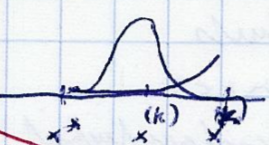
\includegraphics[width=0.4\textwidth]{figures/abbruchkriterium.png}
  \caption{Abbruchkriterium Fixpunktiteration}
\end{figure}

\subsection{Bestimmung von Nullstellen reeller Funktionen}
Gesucht: $x^* \in [a,b]$ mit $f(x^*) = 0$\\
Ist $f(a)f(b) < 0$ und $f$ stetig
\begin{figure}[htbp]
  \centering
  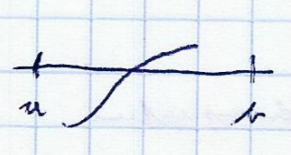
\includegraphics[width=0.4\textwidth]{figures/nst_bsp.png}
  \caption{Beispiel einer Nullstelle}
\end{figure}
$\Rightarrow \exists\; x^* \in (a,b):\;f(x^*) = 0$\\
Einfache (aber langsame) Methode: Bisektionsverfahren\\
Definiere $(a_k, b_k)_{k \in \mathbb{N}_0}$ induktiv durch
\begin{align*}
  (a_0, b_0) =& (a, b)\\
  c_k :=& \frac{a_k + b_k}{2}\\
  (a_{k+1}, b_{k+1}) :=& \begin{cases}
    (a_k, c_k) &\mbox{falls} f(a_k)f(c_k) < 0\\
    (c_k, b_k) &\mbox{sonst}
  \end{cases}
\end{align*}
lineare Konvergenz $(x^*, x^*)$\\
\matlab{fzero} (basierend auf Bisektion)\\
Nur eine Nullstelle und auch keine Information ob es mehrere gibt.\\

Bestimmung der Nullstellen von Polynomen\\
$p(x) = x^n + a_{n-1}x^{n-1} + \ldots + a_0 \Leftrightarrow$ äquivalentes Eigenwertproblem (Begleitmatrix)

\subsection{Newton-Verfahren und seine Varianten}
Zunächst sei $n=1: \quad f:\;(a,b) \rightarrow \mathbb{R}, x^* \in (a,b)$ (unbekannt) mit $f(x^*) = 0$\\
Ziel: Näherungsweise Bestimmung von $x^*$\\
Ansatz: Sei $x^{(k)}$ gegebene Näherung von $x^*$
\begin{enumerate}[i)]
  \item Verwende lineare Approximation von $g$ und $f$ in $x^{(k)}$
  \item Bestimme $x^{(k+1)}$ als Nullstelle von $g$
  \begin{figure}[htbp]
    \centering
    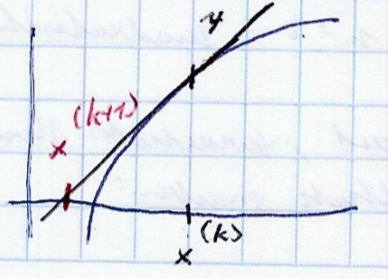
\includegraphics[width=0.4\textwidth]{figures/naeherung_nst.png}
    \caption{Linearisierte Funktion $g$}
  \end{figure}
\end{enumerate}
Implementierungen:
\begin{itemize}
  \item LAPACK (kleine vollbesetzte Matrizen)
  \item ARPACK (größere dünnbesetzte Matrizen)
\end{itemize}
D.h.
\begin{align*}
  f(x) &= \underbrace{f(x^{(k)} + f'(x^{(k)})(x - x^{(k)})}_{=: g(x)} + \LandauO\left( (x - x^{(k)})^2 \right)\\
  0 &\mustbe g(x^{(k+1)})\\
  \mathbin{\textcolor{rot}{x^{k+1} = x^k - [f(x^k)]^{-1} f(x^k) }}\tag{\textcolor{rot}{Newton-Verfahren für $f(x)=0$}}\\
  \text{Auch gültig in } \rn &\quad f'(x^{(k)})\ldots\text{Jacobi-Matrix}
\end{align*}
\satz: Sei $f:\;M \subset \rn \rightarrow \rn$ 2-mal stetig differenzierbar und $f(x^*) = $ für $x^* \in M$.\\
Ist $f'(x^*)$ invertierbar, dann ist das Newton-Verfahren lokal quadratisch konvergent.\\
Standard-Newton-Verfahren konvergiert meist nicht oder nicht gegen gewünschte Nullstelle,
wenn Startnäherung $x^{(0)}$ nicht nahe genug bei $x^*$ liegt.\\
Ausweg: ``Globalisierungstechniken'' (``gedämpfte Newton-Verfahren'')
\begin{align*}
  x^{(k+1)} = x^{(k)} - \textcolor{rot}{\lambda_k}[f'(x^{(k)})]^{-1} f(x^{(k)}
\end{align*}
$\lambda_k$ (Dämpfer, Schrittweite) wird so gewählt (und kann so gewählt werden), dass
\begin{itemize}
  \item $\norm{f(x^{(k+1)}} < \norm{f(x^{(k)}}$
  \item $\norm{f(x^{(k+1)}}$ möglichst klein in einem gewissen Bereich
    \begin{itemize}
      \item line search
      \item trust region %TODO stimmt?
      \item Levenberg-Marquardt
    \end{itemize}
\end{itemize}
Konvergenz gegen $x^*$ ist NICHT gewährleistet.\\
\matlab{fsolve}

